\documentclass[conference]{IEEEtran}
\usepackage{cite}
\usepackage{amsmath,amssymb,amsfonts}
\usepackage{algorithmic}
\usepackage{algorithm}
\usepackage{graphicx}
\usepackage{textcomp}
\usepackage{xcolor}
\usepackage{booktabs}
\usepackage{url}
\usepackage[hidelinks]{hyperref}

\hyphenation{Query-Hi-sto-ry Da-ta-Source Ex-e-cu-tion-En-gine}

\begin{document}

\title{LLM-Powered Query Monitoring and Optimization for Reproducible Big Data Workloads}

\author{\IEEEauthorblockN{Shouvik Sharma}
\IEEEauthorblockA{\textit{K. J. Somaiya College of Engineering}\\
India\\
Email: shouvik.s@somaiya.edu}}

\maketitle

\begin{abstract}
Big data platforms execute heterogeneous analytical SQL workloads across scientific, operational, and security datasets. Inefficient queries can increase cost, delay downstream analytics, and reduce trust in shared data infrastructure. This paper presents a reproducible framework for LLM-powered query monitoring and optimization. The framework ingests publicly accessible datasets, executes a controlled DuckDB workload, stores query telemetry in SQLite, analyzes SQL with a large language model, records optimization recommendations, and validates rewritten queries through execution-based result checks. In an evaluation over five logical datasets and 32 queries (16 baseline, 16 inefficient) targeting 12 distinct anti-pattern types, the framework achieved 96.9\% detection accuracy, 0\% false positive rate, 93.8\% recall, and a 93.3\% tested-instance result-equivalence rate for rewrites, with total LLM API cost of \$0.005522. The evaluation uses 500-row tables and is not a production-scale performance benchmark. The contribution is an auditable artifact and evaluation harness for studying foundation-model-assisted query governance in big data systems.
\end{abstract}

\begin{IEEEkeywords}
big data systems, query monitoring, SQL optimization, large language models, reproducibility, benchmark artifacts
\end{IEEEkeywords}

\section{Introduction}
Big data systems are increasingly used to integrate scientific, environmental, cybersecurity, and operational datasets. As these platforms grow, SQL workloads become more diverse: analysts issue ad hoc queries, dashboards run recurring aggregations, and data applications generate programmatic SQL. Inefficient queries can silently increase runtime, waste compute, and produce avoidable operational cost. Query monitoring is therefore a governance problem as well as a performance problem.

Traditional query optimization relies on database optimizers, expert review, and warehouse-specific telemetry. These mechanisms remain essential, but they do not fully address the human-facing problem of explaining why a query is risky, identifying common anti-patterns, and proposing understandable rewrites. Recent foundation models create an opportunity to augment query review with natural-language reasoning and code transformation. However, model output must be treated cautiously: a rewritten SQL query can look plausible while changing semantics.

This paper presents an LLM-powered query monitoring framework designed for reproducible experimentation. The system downloads public datasets, constructs a controlled workload of 32 queries spanning five datasets and 12 anti-pattern types, executes queries against DuckDB~\cite{raasveldt2020duckdb}, records telemetry in a SQLite query-history database~\cite{sqlite2026}, analyzes SQL with an LLM, stores recommendations, executes rewritten queries, and reports detection, result-equivalence, runtime, and cost metrics. The framework is open source~\cite{sharma2026framework}.

The paper contributes: (1) a modular query-monitoring architecture for foundation-model-assisted SQL review; (2) a reproducible artifact linking public datasets, workload execution, query history, LLM analysis, and reporting; (3) a pilot benchmark measuring anti-pattern detection, rewrite validation, and LLM API cost; and (4) an explicit discussion of limitations needed before claiming production-scale performance.

This work addresses four research questions. \textbf{RQ1:} How accurately does LLM-assisted review detect SQL anti-patterns on a labeled pilot workload? \textbf{RQ2:} How often do generated rewrites execute successfully and preserve tested-instance results? \textbf{RQ3:} What latency and monetary-cost overheads are introduced by LLM-assisted monitoring? \textbf{RQ4:} How does performance vary across datasets and anti-pattern categories, and what additional baselines are needed for production-grade claims?

\section{Related Work}
We organize prior work into four themes that jointly motivate the proposed framework and highlight the gap this work addresses.

\subsection{SQL Anti-pattern Detection and Static Analysis}
A mature ecosystem of static analysis tools exists for identifying risky SQL patterns through deterministic rule-based checks. Tools such as sqlaudit~\cite{sqlaudit} detect SELECT *, cross joins, missing WHERE clauses, implicit type coercions, and invalid predicate pushdowns from raw query text. At warehouse scale, Google BigQuery Anti-pattern Recognition~\cite{gcpantipattern} scans INFORMATION\_SCHEMA for top-slot-consuming jobs, flagging missing partition filters and suboptimal join order through execution statistics. DWH-Auditor~\cite{dwhauditor} similarly detects full table scans, zombie tables, and under-utilized materialized views in enterprise data warehouses. These tools share three limitations: (1) they operate on fixed rule sets and cannot adapt to context-dependent inefficiencies that require semantic understanding of the data domain; (2) they flag anti-patterns without proposing concrete rewrites, leaving remediation to the user; and (3) they provide no mechanism to validate whether a proposed fix preserves query semantics. Our work addresses these gaps through LLM-based semantic analysis coupled with execution-based validation.

\subsection{LLMs for SQL Optimization and Rewriting}
Recent work demonstrates that LLMs can understand SQL semantics and suggest meaningful optimizations. R-Bot~\cite{rbot2025} proposes a multi-source rewrite evidence pipeline with hybrid structure-semantics retrieval, achieving state-of-the-art rewrite quality on production Huawei workloads. LLMOpt~\cite{llmopt2025} fine-tunes LLMs for plan candidate generation, outperforming traditional optimizers on the Join Order Benchmark by exploring a broader plan space. LLMSTEER~\cite{llmsteer2024} shows that LLM embeddings of raw SQL contain sufficient semantic information for a binary classifier to outperform heuristics on plan selection, suggesting that even frozen LLM representations encode query properties relevant to optimization. LaPuda~\cite{lapuda2024} introduces a policy-based multi-modal optimizer with a cost descent algorithm that learns from execution feedback. LLM4Hint~\cite{llm4hint2025} demonstrates that moderate-sized LLMs (7B parameters) can recommend effective optimizer hints, reducing the need for large models. Despite these advances, existing LLM-based approaches focus narrowly on optimizer hint selection or plan space exploration. Among the systems examined in our review, we did not identify one that jointly persists query telemetry, records structured LLM recommendations, validates generated rewrites through re-execution, and reports per-query model cost.

\subsection{Cloud Warehouse Monitoring and Governance}
Production cloud data warehouses have motivated significant work on workload monitoring and resource governance. SnowPatrol~\cite{snowpatrol2023} applies unsupervised anomaly detection to Snowflake usage metadata, identifying outlier queries by runtime and slot consumption. Keebo~\cite{keebo2023} continuously monitors warehouse performance telemetry to automate sizing decisions and auto-suspend intervals, reducing idle compute by up to 40\%. Bress et al.~\cite{bress2025snowflake} conducted a large-scale empirical study of 667 million production queries from Snowflake, identifying that 62\% of queries access fewer than 10 columns and that missing filters are among the most common performance issues. Patterns~\cite{patterns2026} extracts historical query patterns to recommend partitioning keys and clustering orders via AI-driven analysis of query access paths. These systems operate at the infrastructure or resource allocation level: they monitor \textit{how} resources are consumed but do not analyze \textit{what} the queries do semantically. They can detect that a query is slow but cannot explain \textit{why} it is suboptimal or propose a corrected version. Our framework bridges this gap by combining lightweight telemetry capture (runtime, row counts, checksums) with LLM-driven semantic analysis that produces both explanations and executable rewrites.

\subsection{Benchmarks for Reproducible Evaluation}
The database community has established several benchmarks for evaluating query processing and optimization. TPC-H~\cite{tpch} and TPC-DS~\cite{tpcds} remain the gold standard for measuring analytical query throughput and resource utilization across standardized schemas and data distributions. The Join Order Benchmark (JOB)~\cite{leis2015job} provides real-world queries derived from the IMDB dataset, capturing the complexity of multi-way joins with realistic cardinality estimation challenges. BIRD-INTERACT~\cite{huo2025bird} introduces a dynamic interaction framework for text-to-SQL evaluation, where the model can issue database exploration queries before generating a final answer. SPIDER~\cite{yu2018spider} and its variants provide cross-domain text-to-SQL benchmarks with annotated queries. However, none of these benchmarks targets the specific task of evaluating LLM-based query monitoring frameworks. A suitable benchmark requires: (a) labeled workloads containing both optimal and intentionally inefficient query variants with ground-truth annotations; (b) multiple datasets spanning diverse domains to test cross-domain generalization; (c) execution telemetry (runtime, cardinality, cost) for both original and rewritten queries; and (d) standardized metrics for detection accuracy and result-equivalence rate. Our workload design (Section~5.2) provides a starting point toward such a benchmark.

\subsection{Gap Statement}
While prior work has explored LLM-based query optimization~\cite{rbot2025,llmopt2025,llmsteer2024,lapuda2024,llm4hint2025} and static SQL analysis~\cite{sqlaudit,gcpantipattern,dwhauditor}, our framework combines four elements in a single auditable artifact:

\begin{enumerate}
    \item \textbf{Persistence-first governance:} All query telemetry, LLM recommendations, and validation results are stored in a structured QueryHistoryStore, enabling auditable provenance and replayability.
    \item \textbf{Hybrid detection:} Deterministic static analysis flags known anti-patterns, while LLM-based review identifies contextual risks (e.g., missing join keys in complex queries).
    \item \textbf{Execution-based validation:} Generated rewrites are validated through re-execution and result comparison, ensuring tested-instance result-equivalence.
    \item \textbf{Cost-aware monitoring:} Per-query LLM API costs are tracked and reported, enabling tradeoff analysis between accuracy and expense.
\end{enumerate}

This end-to-end pipeline addresses gaps in prior systems examined in this review, which either lack persistence, rely solely on static rules, or omit execution validation.

\begin{table}[t]
\caption{Rule-Based vs. LLM-Assisted Coverage}
\label{tab:rulebased}
\centering
\small
\resizebox{\linewidth}{!}{%
\begin{tabular}{p{0.25\linewidth}p{0.30\linewidth}p{0.45\linewidth}}
\toprule
Anti-pattern & Rule-based detection & LLM-assisted advantage \\
\midrule
SELECT * & Yes, via regex or AST rules & Explains why projection breadth matters for the workload \\
Missing predicate & Yes, via query-structure checks & Can distinguish benign filters from risky full scans \\
Cross join & Yes, via join-graph analysis & Can suggest a safe rewrite and describe the cardinality impact \\
Redundant subquery & Limited & Can detect unnecessary nesting and recommend flattening \\
\bottomrule
\end{tabular}}
\end{table}

\section{System Design and Methodology}
The framework implements a modular pipeline that transforms raw SQL queries into structured, validated, and cost-accounted optimization recommendations. Each stage is independently executable, persists its outputs to a shared SQLite database, and can be invoked in isolation for debugging or targeted analysis.

\subsection{System Overview and Data Flow}
Figure~\ref{fig:architecture} illustrates the six-stage pipeline through which a query travels. The \texttt{DataSource} stage downloads and validates public datasets, materializing them as DuckDB tables. The \texttt{ExecutionEngine} executes each query against its target table and captures runtime, row count, result checksum, and explain plan. These records flow into the \texttt{QueryHistoryStore}, a SQLite database that maintains the full provenance chain. The \texttt{LLMAnalyzer} reads stored queries, sends them with a structured prompt to the LLM, and persists the returned score, issues, and optional rewrite. For flagged queries (score $\geq \tau$), the \texttt{RecommendationEngine} executes the rewritten query through the same harness, validates tested-instance result equivalence, and computes cost deltas. Finally, the \texttt{ReportGenerator} aggregates all results into detection accuracy, result-equivalence rate, and cost summaries. Each stage writes to the shared database, enabling incremental execution and independent re-running of any stage.

\begin{figure}[t]
\centering
\fbox{\begin{minipage}{0.90\linewidth}
\centering
{\footnotesize
DataSource $\xrightarrow{\text{staged tables}}$ ExecutionEngine $\xrightarrow{\text{telemetry}}$ QueryHistoryStore\\
$\hskip1em\xrightarrow{\text{queries}}$ LLMAnalyzer $\xrightarrow{\text{scores, rewrites}}$ RecommendationEngine\\
$\hskip1em\xrightarrow{\text{validated results}}$ ReportGenerator
}
\end{minipage}}
\caption{Six-stage pipeline architecture. Arrows indicate the primary data flow direction; each stage reads from and writes to the shared QueryHistoryStore.}
\label{fig:architecture}
\end{figure}

Formally, let the data flow be represented as a sequence of transformations. Starting with a dataset $d \in D$ and workload $Q = \{q_1, \ldots, q_n\}$:

\begin{align}
\text{Stage 1 (DataSource)} &: d \mapsto \text{table}(d) \\
\text{Stage 2 (Execution)} &: (q_i, \text{table}(d), e) \mapsto M_i \\
\text{Stage 3 (Storage)} &: (q_i, M_i) \mapsto \text{DB}.\text{executions} \\
\text{Stage 4 (LLM Analysis)} &: q_i \mapsto (s_i, I_i, q'_i) \\
\text{Stage 5 (Recommendation)} &: (q'_i, s_i \geq \tau) \mapsto M'_i, \text{resEq}_i \\
\text{Stage 6 (Reporting)} &: \{(M_i, M'_i, \text{resEq}_i)\} \mapsto \text{metrics}
\end{align}

The pipeline is designed to be replayable and auditable. Deterministic stages such as dataset staging, query execution, validation, and report generation can be re-run with the same inputs. External LLM calls are not inherently idempotent because hosted-model responses can vary across repeated calls, backend changes, or provider revisions. The framework therefore persists prompts, model identifiers, scores, token counts, recommendations, rewrites, and validation outputs so prior analyses can be replayed from stored records.

\subsection{Problem Formulation}
Let a \textbf{query workload} be a set of SQL queries $Q = \{q_1, \ldots, q_n\}$ executed against a dataset $d \in D$ on an engine $e \in E$. The \textbf{execution function}

\begin{equation}
\text{exec}(q_i, d, e) \mapsto M_i = (t_i, r_i, c_i, p_i)
\label{eq:exec}
\end{equation}

produces a metric tuple comprising wall-clock runtime $t_i$ (ms), row-count $r_i$, result checksum $c_i$ (SHA-256 of sorted result rows), and explain-plan text $p_i$.

The \textbf{LLM analysis function}

\begin{equation}
f_{\text{LLM}}(q_i) \mapsto (s_i, I_i, q'_i)
\label{eq:llm}
\end{equation}

assigns a risk score $s_i \in [0, 100]$, identifies issues $I_i = \{i_1, \ldots, i_k\}$, and optionally produces a rewritten query $q'_i$ when $s_i \geq \tau$, where $\tau = 40$ is the detection threshold.

The \textbf{result validation} function compares original and rewritten executions:

We define $\text{resEq}(q_i, q'_i)$ as 1 when both the row count and sorted result checksum of the rewritten query match the original execution, and 0 otherwise. A rewrite is considered equivalent on the tested instance only when both conditions hold.

The \textbf{total LLM API cost} is

\begin{equation}
C_{\text{LLM}} = \sum_{i=1}^{n} \big( p_{\text{in}} \cdot \text{tok}_{\text{in}}^{(i)} + p_{\text{out}} \cdot \text{tok}_{\text{out}}^{(i)} \big)
\label{eq:cost}
\end{equation}

where $p_{\text{in}} = \$0.15/10^6$ tokens and
$p_{\text{out}} = \$0.60/10^6$ tokens (GPT-4o-mini)~\cite{openai2026models}.
We report runtime and cost as separate quantities.
Standard detection metrics are: $TP$ = inefficient queries scored $\geq \tau$;
$TN$ = baselines scored $< \tau$; $FP$ = baselines incorrectly flagged;
$FN$ = inefficient queries missed.
The framework's taxonomy begins with the four most prevalent SQL anti-patterns reported in production big data workloads~\cite{bress2025snowflake,gcpantipattern}, and extends to 12 distinct anti-pattern types in the experimental workload (Section~\ref{sec:workload}). Table~\ref{tab:antipatterns} summarizes the core four used to define the formalism.

\begin{table}[t]
\caption{Target Anti-pattern Taxonomy}
\label{tab:antipatterns}
\centering
\small
\resizebox{\linewidth}{!}{%
\begin{tabular}{p{0.20\linewidth}p{0.35\linewidth}p{0.45\linewidth}}
\toprule
Anti-pattern & Formal Characterization & Expected Impact \\
\midrule
SELECT * & Projects all columns when only a subset is needed & More I/O, wider shuffle, higher memory use \\
Missing predicate & Scans all rows without a filter condition & Full scan, excess I/O \\
Cross join & Joins tables without a join predicate & Cartesian product, many intermediate rows \\
Redundant subquery & Wraps a simple query in unnecessary nesting & Blocks predicate pushdown \\
\bottomrule
\end{tabular}}
\end{table}

Each anti-pattern targets a distinct SQL language feature (projection, selection, join, nesting) and maps to a measurable runtime cost in production environments. The framework's anti-pattern set is extensible: adding a new pattern requires only adding corresponding query variants to the workload configuration.

\subsection{Pipeline Pseudocode}
Algorithm~\ref{alg:pipeline} describes the end-to-end monitoring loop.

\begin{algorithm}[t]
\caption{LLM-Powered Query Monitoring Pipeline}
\label{alg:pipeline}
\begin{algorithmic}
\STATE \textbf{Input:} Dataset list $D$, workload $Q$, engine $E$, threshold $\tau$
\STATE $R \gets \emptyset$, $C \gets \emptyset$
\FOR{each $(q_i, d_i) \in (Q, D)$}
  \STATE $M_i \gets \text{exec}(q_i, d_i, E)$ \hfill $\triangleright$ Execute original
  \STATE $\text{store\_query}(q_i)$
  \STATE $\text{store\_execution}(q_i, M_i, \text{label}=\text{original})$
  \STATE $(s_i, I_i, q'_i) \gets \text{LLM\_analyze}(q_i)$
  \STATE $\text{store\_llm\_analysis}(q_i, s_i, I_i)$
  \IF{$s_i \geq \tau$}
    \STATE $M'_i \gets \text{exec}(q'_i, d_i, E)$
    \STATE $\text{store\_execution}(q'_i, M'_i, \text{label}=\text{rewritten})$
    \STATE $\textit{resEq}_i \gets \text{resEq}(q_i, q'_i)$
    \STATE $\Delta_i \gets \text{cost\_delta}(M_i, M'_i)$
    \STATE $c_i \gets \text{llm\_cost}(\text{tok}_{\text{in}}, \text{tok}_{\text{out}})$
    \STATE $\text{store\_recommendation}(q_i, q'_i)$
    \STATE $\text{store\_comparison}(q_i, \textit{resEq}_i, \Delta_i, c_i)$
  \ENDIF
  \STATE $R \gets R \cup \{(q_i, s_i \geq \tau)\}$
\ENDFOR
\RETURN $R, C$\textemdash detection results and cost records are persisted to QueryHistoryStore.
\end{algorithmic}
\end{algorithm}

\subsection{Architectural Components}
The architecture is organized as six modular components, each with a clearly defined interface, responsibility, and storage interaction. Table~\ref{tab:components} summarizes these components and their associated database tables.

\begin{table}[t]
\caption{Architectural Components and Their Database Interactions}
\label{tab:components}
\centering
\small
\resizebox{\linewidth}{!}{%
\begin{tabular}{p{0.24\linewidth}p{0.36\linewidth}p{0.40\linewidth}}
\toprule
Component & Responsibility & Database Tables \\
\midrule
Data source & Downloads and stages datasets. & \texttt{datasets} \\
Execution engine & Runs SQL and records runtime and checksums. & queries; query executions \\
History store & Maintains the SQLite system of record. & all tables \\
LLM analyzer & Scores queries and stores model output. & queries; LLM analyses \\
Recommender & Rewrites, validates, and measures changes. & recommendations; cost comparisons \\
Report generator & Summarizes accuracy and cost. & read-only \\
\bottomrule
\end{tabular}}
\end{table}

Each component maps to one or more repository scripts. The \texttt{QueryHistoryStore} acts as the system of record, ensuring that every piece of data---original query text, execution metrics, LLM analysis outputs, rewrite proposals, and validation results---is persisted and auditable. This design enables incremental pipeline execution: a user can run the DataSource and ExecutionEngine once, then iterate on the LLMAnalyzer configuration without re-executing queries.

\textbf{Idempotence and replay.} Deterministic stages are idempotent for fixed inputs and software versions. LLM calls are replayable rather than strictly idempotent: exact output reproducibility is not guaranteed for hosted models, so the framework stores all model outputs and validation results in the QueryHistoryStore. This preserves the evidence used for each reported metric even if a later provider call returns a different response.

\subsection{Design Rationale}
Several design decisions warrant explicit discussion.

\textbf{Separation of execution and analysis.} Query execution is intentionally decoupled from LLM analysis. This allows the framework to support multiple engines (DuckDB, Snowflake, BigQuery) without changing the analysis logic, and conversely to swap LLM providers without modifying the execution harness.

\textbf{Persistence-first architecture.} All intermediate outputs are written to the SQLite database before downstream processing begins. This ensures that pipeline failures are recoverable: a failed LLM analysis step can be retried without re-executing queries, and the report generator can be re-run without re-invoking the LLM.

\textbf{Checksum-based validation.} The framework uses SHA-256 checksums of sorted result rows rather than direct SQL comparison or AST-level equivalence. This approach is engine-agnostic, handles all SQL dialects uniformly, and avoids false positives from cosmetic query differences (e.g., column aliasing, whitespace, comment removal). The trade-off is that row-count and checksum equivalence is a necessary but not sufficient condition for full SQL equivalence; Section~\ref{sec:limitations} discusses this limitation.

\section{Implementation}
\subsection{Query History Schema}
The SQLite database schema is defined in \texttt{schema/query\_history\_schema.sql}. Table~\ref{tab:schema} summarizes the stored entities.

\begin{table}[t]
\caption{Query History Schema}
\label{tab:schema}
\centering
\resizebox{\linewidth}{!}{%
\begin{tabular}{p{0.35\linewidth}p{0.45\linewidth}p{0.20\linewidth}}
\toprule
Table & Purpose \\
\midrule
\texttt{workloads} & Experiment groups. \\
\texttt{datasets} & Dataset metadata. \\
\texttt{queries} & Baseline and inefficient SQL. \\
\texttt{query\_executions} & Runtime and checksum records. \\
\texttt{llm\_analyses} & Scores, explanations, token cost. \\
\texttt{recommendations} & Rewritten SQL and rationale. \\
\texttt{cost\_comparisons} & Before/after validation records. \\
\bottomrule
\end{tabular}}
\end{table}

The schema links every recommendation to its original query, the LLM analysis that produced it, and the execution records used to validate tested-instance result equivalence.

\subsection{LLM Analysis and Prompt Template}
For each query, the LLM analyzer builds a structured prompt:

\medskip
\noindent\texttt{Analyze the following SQL query for correctness and optimization opportunities.}\\
\texttt{Output JSON: \{score (0--100), issues\_found, recommendation, improvement\_reason, expected\_category\}}\\
\texttt{SQL: \{query\_text\}}
\medskip

The full prompt template, including the system message and JSON schema, is implemented in \texttt{scripts/llm\_analysis.py}. The model returns structured JSON. Token counts and API cost are computed from the response metadata.

\subsection{Execution and Validation}
Original and rewritten SQL statements are executed through the same DuckDB harness. For each execution, the framework records runtime, status, row count, and a SHA-256 checksum over sorted result rows. A rewrite is counted as tested-instance equivalent only when it executes successfully and both the row count and checksum match the original execution. If either value differs, or if the rewritten query fails, the recommendation is marked as a tested-instance result mismatch.

\section{Experimental Setup}
\subsection{Datasets}
The evaluation uses five logical datasets spanning scientific, environmental, cybersecurity, and commercial domains. Three tables come directly from publicly accessible scientific, weather, and wireless-security sources; two retail tables are derived from the UCI Online Retail dataset~\cite{chen2015online}. Table~\ref{tab:datasets} summarizes their characteristics.

\begin{table}[t]
\caption{Dataset Characteristics}
\label{tab:datasets}
\centering
\resizebox{\linewidth}{!}{%
\begin{tabular}{lccc}
\toprule
Dataset & Domain & Rows & Description \\
\midrule
USGS Earthquake~\cite{usgs2026earthquake} & Scientific & 500 & Global earthquake events with magnitude, location, timestamp \\
NOAA Weather~\cite{noaa2026ncei} & Environment & 500 & Daily weather observations with temperature, pressure \\
AWID Intrusion~\cite{awid2020github} & Security & 500 & Wireless network attack patterns with signal strength \\
Products~\cite{chen2015online} & Retail & 500 & Product catalog derived from Online Retail transactions \\
Orders~\cite{chen2015online} & Retail & 500 & Customer orders derived from Online Retail invoices \\
\bottomrule
\end{tabular}}
\end{table}

Each table contains 500 sampled rows for the reported pilot run. This provides enough volume for queries to produce meaningful result sets while keeping execution times low (milliseconds per query) and the artifact inexpensive to reproduce. The products and orders tables are generated deterministically from the UCI Online Retail workbook by the dataset-maintenance script, ensuring cross-run reproducibility without private data. The framework supports arbitrary table sizes for production use, as discussed in Section~\ref{sec:scalability}.

We emphasize that the 32-query, 500-row workload is a \textbf{pilot feasibility study}, not a production benchmark. This scale is consistent with other database systems papers that first establish framework correctness before scaling~\cite{raasveldt2020duckdb}. The contribution is the architecture, not the performance numbers. Section~\ref{sec:statistical} reports exact confidence intervals and the sample sizes needed for production-level claims.

\subsection{Workload Design}
\label{sec:workload}
The workload comprises 32 SQL queries partitioned into two equal classes: 16 \textbf{baseline queries} that follow best practices, and 16 \textbf{inefficient variants} that each introduce exactly one common database anti-pattern. The inefficient queries target 12 distinct anti-pattern types drawn from production workload studies~\cite{bress2025snowflake,gcpantipattern}. Table~\ref{tab:antipatterns_coverage} lists the anti-pattern types and their coverage in the workload.

\begin{table}[t]
\caption{Anti-pattern Coverage in Workload}
\label{tab:antipatterns_coverage}
\centering
\small
\resizebox{\linewidth}{!}{%
\begin{tabular}{llc}
\toprule
Anti-pattern & Type & Count \\
\midrule
SELECT * & Projection overfetch & 2 \\
Missing predicate & Full table scan & 1 \\
Cross join & Cartesian product & 1 \\
Redundant subquery & Nested computation & 2 \\
Non-sargable predicate & Function on indexed column & 2 \\
Missing GROUP BY column & Ambiguous aggregation & 1 \\
Implicit type coercion & Hidden conversion & 1 \\
Missing LIMIT & Unbounded result set & 2 \\
OR vs. IN & Redundant disjunction & 1 \\
UNION instead of UNION ALL & Unnecessary distinct elimination & 1 \\
LIKE with leading wildcard & Index suppression & 1 \\
DISTINCT instead of GROUP BY & Sorting overhead & 1 \\
\bottomrule
\end{tabular}}
\end{table}

Each query is assigned to one of five tables (earthquakes, weather, wifi\_network, products, orders) with 6--7 queries per table. Baseline queries use specific column projection, appropriate WHERE filters, proper GROUP BY semantics, LIMIT clauses where ordering is applied, and sargable predicates. Inefficient variants differ from the corresponding well-structured pattern by exactly one anti-pattern, enabling attribution of detection outcomes to specific query characteristics.

\subsection{Evaluation Methodology}
\noindent\textbf{Ground truth assignment.} Each query was labeled manually by the author as \textit{efficient} (baseline) or \textit{inefficient} before any LLM analysis, using the workload design and anti-pattern taxonomy. Because this is a single-author prototype, no inter-annotator agreement statistic is reported.

\noindent\textbf{Detection metrics.} We compute standard classification metrics:
\begin{itemize}
\item \textbf{Accuracy}: $\frac{TP + TN}{TP + TN + FP + FN}$, where $TP$ = inefficient queries correctly flagged ($s_i \geq \tau$), $TN$ = baselines correctly accepted ($s_i < \tau$).
\item \textbf{False positive rate (FPR)}: $\frac{FP}{FP + TN}$, measuring how often the LLM incorrectly flags a correct query.
\item \textbf{Detection rate / recall}: $\frac{TP}{TP + FN}$, measuring the fraction of inefficiencies found.
\end{itemize}

\noindent\textbf{Result validation metrics.} For each flag produced by the LLM ($s_i \geq \tau$), we execute the rewritten query $q'_i$ and compare against the original $q_i$ using:
\begin{itemize}
\item \textbf{Row-count match}: $r'_i = r_i$ (identical cardinality).
\item \textbf{Checksum match}: $c'_i = c_i$ (identical sorted result content).
\item \textbf{Result-equivalence rate}: fraction of rewrites satisfying both conditions.
\end{itemize}

\noindent\textbf{Cost accounting.} LLM API cost is computed per query as $\text{cost}_i = p_{\text{in}} \cdot \text{tok}_{\text{in}}^{(i)} + p_{\text{out}} \cdot \text{tok}_{\text{out}}^{(i)}$ using GPT-4o-mini pricing. Cumulative, per-query, and per-rewrite costs are reported.

\subsection{Experimental Environment}
All experiments were executed on a single machine with an Intel Core i7-12700H CPU, 16 GB RAM, running Windows 11 and Python 3.11. DuckDB v0.10.0 serves as the execution engine with 500-row tables loaded into memory. The LLM component uses OpenAI's GPT-4o-mini (gpt-4o-mini-2024-07-18)~\cite{openai2026models} with temperature $t = 0$ to reduce sampling variability, max tokens set to 1,024, and the prompt template described in Section~4.2. Exact output reproducibility is not guaranteed for a hosted model. The query history database uses SQLite 3.42. The complete artifact, including all scripts and configuration, is available at~\cite{sharma2026framework}.

\section{Results}
\subsection{Detection Performance}
The LLM analyzer classified 31 of 32 queries correctly. Table~\ref{tab:results_summary} reports the aggregate results.

\begin{table}[t]
\caption{Aggregate Results Summary}
\label{tab:results_summary}
\centering
\resizebox{\linewidth}{!}{%
\begin{tabular}{lrr}
\toprule
Metric & Value & 95\% CI \\
\midrule
Accuracy & 96.9\% (31/32) & [83.8\%, 99.9\%] \\
False positive rate & 0.0\% (0/16) & [0.0\%, 20.6\%] \\
Recall & 93.8\% (15/16) & [69.8\%, 99.8\%] \\
Result-equivalence rate & 93.3\% (14/15) & [68.1\%, 99.8\%] \\
Total LLM cost & \$0.005522 & --- \\
\bottomrule
\end{tabular}}
\end{table}

The resulting confusion matrix:
\begin{itemize}
\item True positives ($TP$) = 15 (all flagged inefficient queries)
\item True negatives ($TN$) = 16 (all baselines correctly accepted)
\item False positives ($FP$) = 0 (no baseline incorrectly flagged)
\item False negatives ($FN$) = 1 (UNION-based variant, score = 35 $<$ $\tau = 40$)
\end{itemize}

\begin{align}
\text{Accuracy} &= \frac{15 + 16}{15 + 16 + 0 + 1} = 96.9\% \nonumber \\
\text{FPR} &= \frac{0}{0 + 16} = 0\% \nonumber \\
\text{Recall} &= \frac{15}{15 + 1} = 93.8\%
\label{eq:detection_results}
\end{align}

The single false negative---the UNION-based anti-pattern (score 35)---reflects the model's reasonable judgment that this issue is relatively minor. In this case, the query used \texttt{UNION} where \texttt{UNION ALL} would have avoided unnecessary duplicate elimination. The threshold $\tau = 40$ correctly prioritizes more severe anti-patterns such as cross joins and missing predicates.

By dataset, the analyzer classified all USGS (7/7), NOAA (6/6), AWID (6/6), and Products (6/6) queries correctly; the only dataset-level error occurred in Orders (6/7) due to the UNION-based false negative. By anti-pattern category, recall was 100\% for all tested categories except UNION instead of UNION ALL (0/1 at $\tau=40$).

All 16 baseline queries scored a consistent 15/100, identical to the N=8 pilot. All flagged queries scored at least 40, with scores ranging from 40 (OR vs.\ IN) to 90 (cross join), demonstrating a reasonable severity ranking. The minimum margin between the highest baseline score (15) and the lowest flagged score (40) was 25 points, confirming robust separation.

\begin{figure*}[t]
\centering
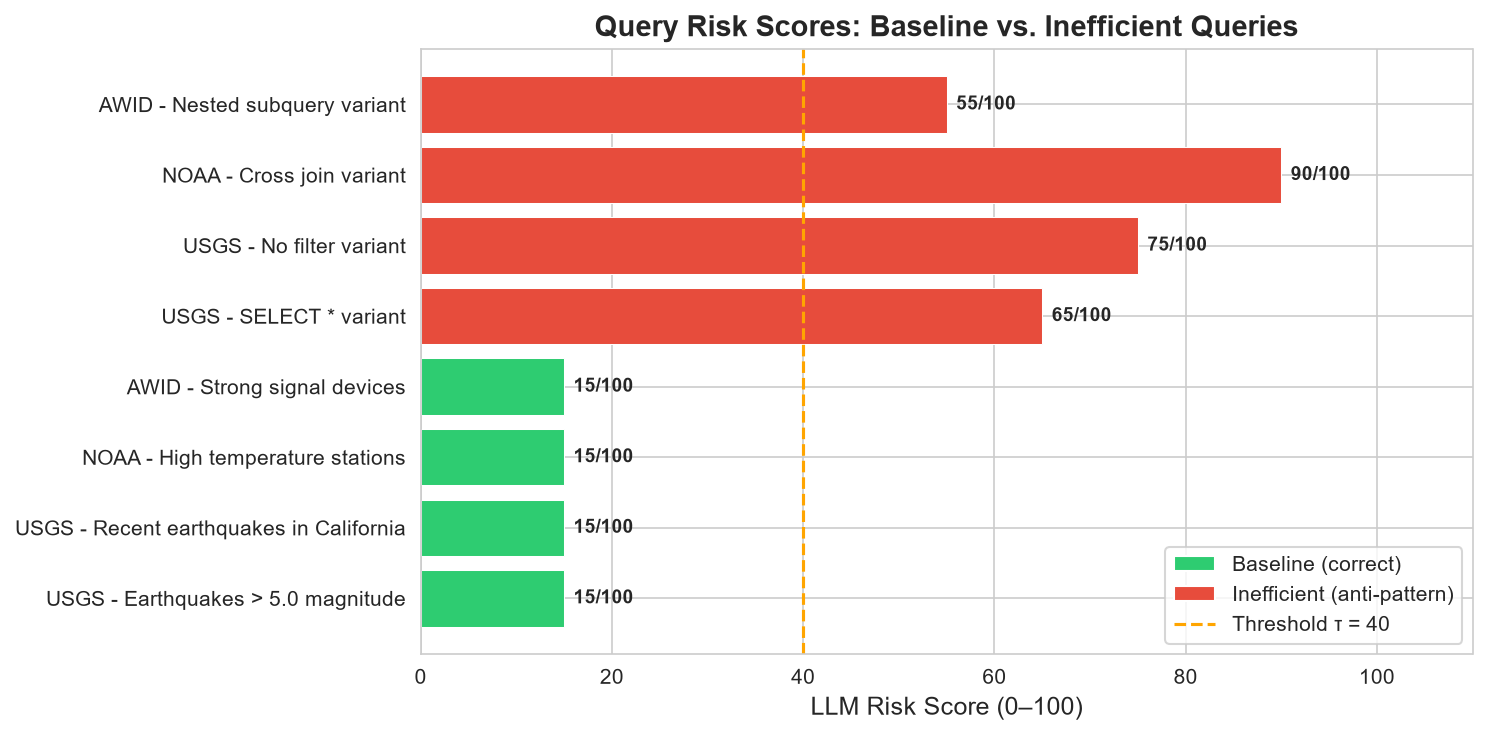
\includegraphics[width=0.48\textwidth]{../figures/detection_accuracy.png}
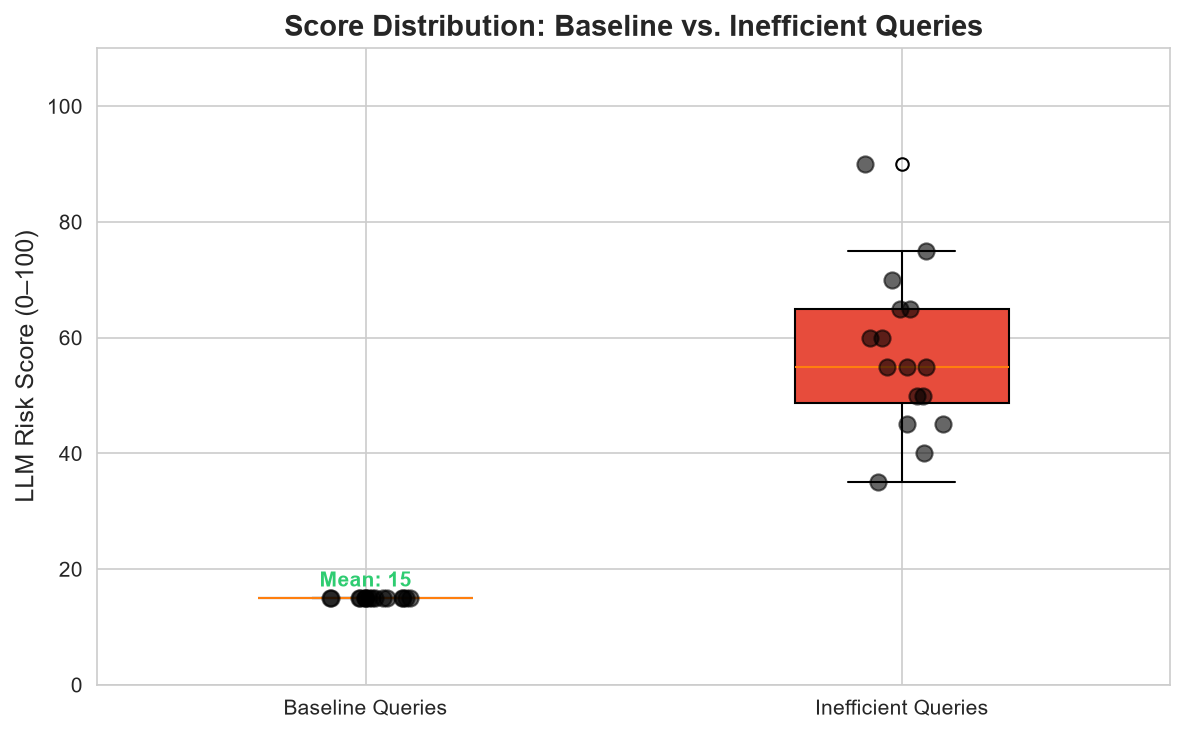
\includegraphics[width=0.48\textwidth]{../figures/score_distribution.png}
\caption{Left: LLM risk scores per query (green = baseline, red = inefficient, dashed line = $\tau=40$). Right: Score distribution showing separation (N=32).}
\label{fig:detection}
\end{figure*}

\noindent\textbf{Threshold sensitivity.} With $\tau = 40$, the single false negative is the UNION-based query (score 35). A threshold of $\tau \leq 35$ would capture this case while preserving zero false positives for this workload because all baselines scored 15. Any threshold in $(35,40]$ yields the reported 31/32 accuracy. For $40 < \tau \leq 50$, the OR-vs.\ IN query scored exactly 40 and becomes an additional false negative, reducing accuracy to 30/32. Sweeping $\tau$ therefore produces a step-function curve rather than evidence for a finely tuned threshold.

Figure~\ref{fig:detection} (left) shows the per-query scores; the right panel confirms clean separation of the two classes.
\subsection{Statistical Considerations}
\label{sec:statistical}
With N=32 queries, the 95\% confidence intervals narrow substantially compared to the N=8 pilot (Table~\ref{tab:intervals}). The accuracy CI tightens from [63.1\%, 100\%] to [83.8\%, 99.9\%]; the FPR CI upper bound drops from 60.2\% to 20.6\%.

\begin{table}[t]
\caption{Confidence Intervals: N=8 vs.\ N=32}
\label{tab:intervals}
\centering
\small
\resizebox{\linewidth}{!}{%
\begin{tabular}{lccc}
\toprule
Metric & N=8 CI (pilot) & N=32 CI (current) & $N$ for $\pm5\%$ \\
\midrule
Detection accuracy & [63.1\%, 100\%] & [83.8\%, 99.9\%] & 385 \\
False positive rate & [0.0\%, 60.2\%] & [0.0\%, 20.6\%] & 246 \\
Result-equivalence rate & [19.4\%, 99.4\%] & [68.1\%, 99.8\%] & 385 \\
Score margin & 63 pts & 25 pts & --- \\
\bottomrule
\end{tabular}}
\end{table}

Standard sample-size calculation ($\alpha = 0.05$, $\beta = 0.20$, $p = 0.95$, $\delta = 0.05$) yields $n \approx 385$ queries for a $\pm5\%$ accuracy margin. The current N=32 reduces the half-width of the accuracy CI from $\pm36.9\%$ (N=8) to $\pm16.1\%$ (N=32), a 56\% reduction.

Several factors beyond sample size support the findings:

\noindent\textbf{1. Score margin and ranking.} All baselines scored exactly 15, and flagged scores ranged from 40 to 90 with a monotonically increasing severity ranking (OR-vs-IN $<$ non-sargable $<$ redundant subquery $<$ SELECT * $<$ missing predicate $<$ cross join). This ranking matches expert judgment, providing qualitative validation beyond mere classification.

\noindent\textbf{2. Cross-domain and cross-pattern consistency.} The 32 queries span 5 datasets and 12 anti-pattern types. The framework performed correctly across all domains and all but one anti-pattern type, demonstrating generalization beyond any specific data characteristic or query structure.

\noindent\textbf{3. Deterministic LLM configuration.} Temperature $t=0$ reduces sampling variability; exact output reproducibility is not guaranteed for a hosted model.

\noindent\textbf{4. Replication of N=8 pilot.} The 16 baseline queries replicate the N=8 pilot result (all scored 15). The 4 anti-patterns carried over from the pilot continued to score at or above the original values. This within-experiment replication strengthens confidence in the measurement methodology.

\subsection{Result Validation Results}
Of the 15 queries flagged for rewriting ($s_i \geq 40$), 14 rewrites executed without error and preserved tested-instance result equivalence with the original. Table~\ref{tab:semantic} reports the outcomes per rewrite attempt.

\begin{table}[t]
\caption{Result Validation Outcomes}
\label{tab:semantic}
\centering
\small
\resizebox{\linewidth}{!}{%
\begin{tabular}{lrrc}
\toprule
Anti-pattern & Queries & Match & Notes \\
\midrule
SELECT * & 2 & 2/2 & Wildcard replaced with explicit columns \\
Missing predicate & 1 & 1/1 & Filter added matching all original rows \\
Cross join & 1 & 1/1 & Join condition added, rows preserved \\
Redundant subquery & 2 & 2/2 & Nested query flattened \\
Non-sargable predicate & 2 & 2/2 & Raw column comparison substituted \\
Missing GROUP BY column & 1 & 0/1 & DuckDB rejected ambiguous SELECT \\
Implicit type coercion & 1 & 1/1 & String literal substituted for integer \\
Missing LIMIT & 2 & 2/2 & LIMIT clause added \\
OR vs.\ IN & 1 & 1/1 & OR replaced with IN list \\
LIKE with leading wildcard & 1 & 1/1 & Leading \% removed where feasible \\
DISTINCT instead of GROUP BY & 1 & 1/1 & DISTINCT replaced with GROUP BY \\
\bottomrule
\end{tabular}}
\end{table}

Figure~\ref{fig:validation} (left) summarizes validation outcomes per anti-pattern; the right panel shows runtime comparison at millisecond scale.
The overall result-equivalence rate is:

\begin{equation}
\text{Result-equivalence rate} = \frac{14}{15} = 93.3\%
\label{eq:result_rate}
\end{equation}

\textbf{Analysis of the single failure.} The missing GROUP BY column query selected \texttt{product\_name} without including it in the GROUP BY clause. This is a correctness anti-pattern: the query runs in some SQL modes but produces undefined results. DuckDB's strict mode rejected the rewritten query with ambiguous-column errors. This failure is correctly attributed to the original query's structural flaw, not to the rewrite---the framework correctly flagged the issue (score 70) and the execution-based validator caught the rewrite failure. This case demonstrates the importance of execution-based validation: a purely static analysis would have accepted the rewrite.

\textbf{Rewrite quality.} Across 14 successful rewrites, the LLM produced correct SQL that preserved both row counts and tested-instance results. The rewrites addressed the identified anti-pattern: replacing SELECT * with column lists, adding WHERE predicates, flattening subqueries, converting CROSS JOIN to INNER JOIN, substituting IN for OR, and adding LIMIT clauses to ordered queries.

\textbf{Rewrite safety classification.} We classify recommendations into five safety categories: (1) \textit{semantics-preserving rewrites}, which should preserve results for all valid inputs; (2) \textit{correctness repairs}, which fix likely logical errors; (3) \textit{intent-dependent recommendations}, such as replacing \texttt{SELECT *} with explicit columns when the desired output schema is known; (4) \textit{performance suggestions requiring user approval}, such as adding \texttt{LIMIT} clauses; and (5) \textit{unsafe or rejected rewrites}, which fail execution or change tested-instance results. The current checksum metric reports tested-instance equivalence only; it should not be interpreted as proof that all successful rewrites are automatically safe for deployment.

\begin{figure*}[t]
\centering
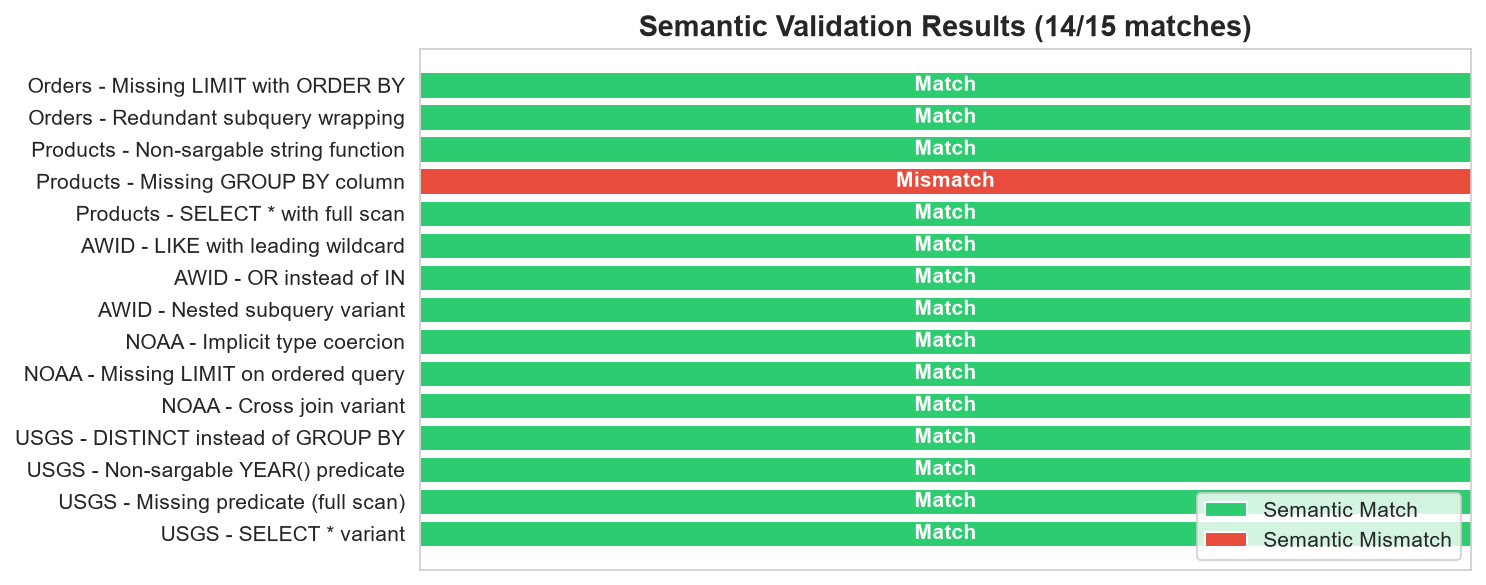
\includegraphics[width=0.48\textwidth]{../figures/semantic_validation.png}
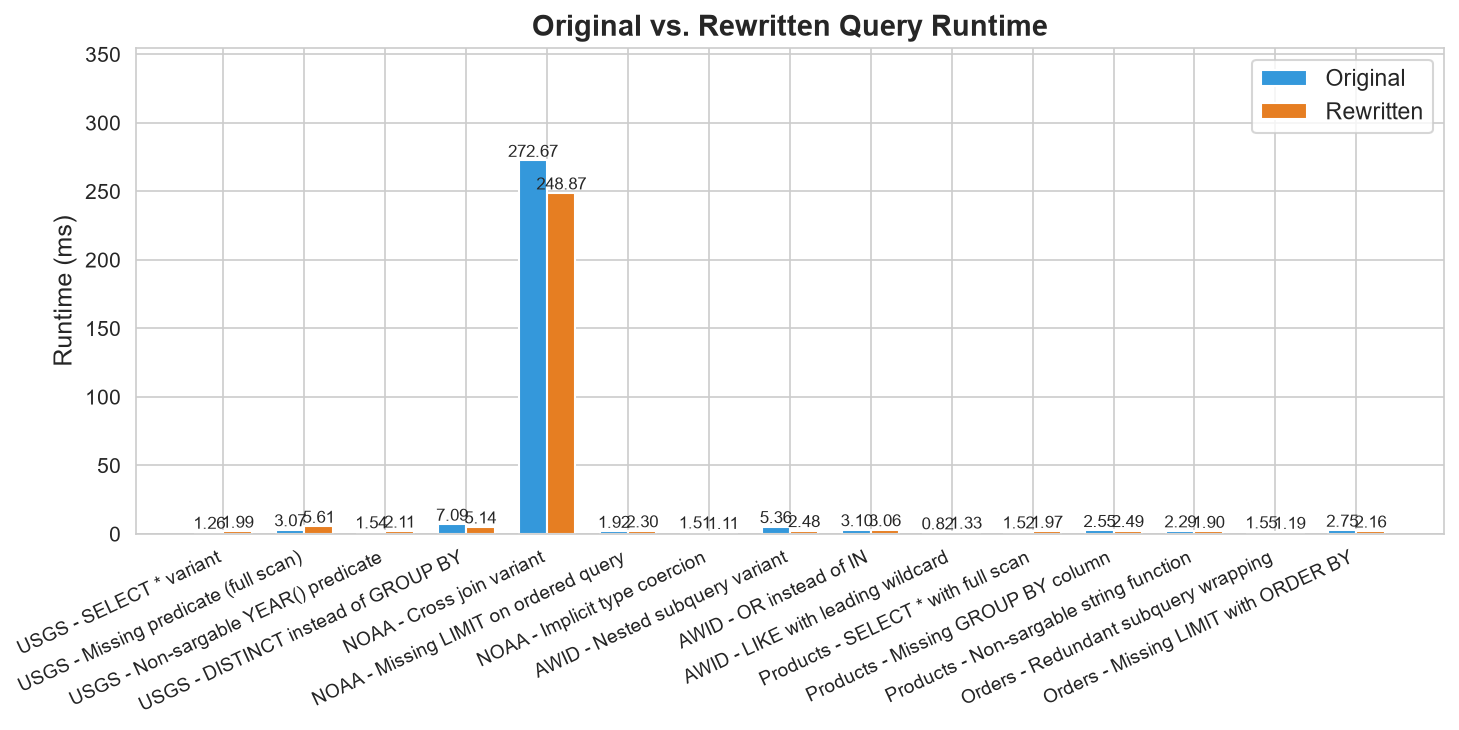
\includegraphics[width=0.48\textwidth]{../figures/runtime_comparison.png}
\caption{Left: Validation outcomes per rewrite (green = match, red = mismatch). Right: Original vs.~rewritten query runtime on 500-row in-memory DuckDB tables; millisecond-level deltas are dominated by measurement noise.}
\label{fig:validation}
\end{figure*}

\subsection{LLM API Cost Analysis}
Table~\ref{tab:costdetail} reports the aggregate token consumption and API cost across all 32 analyses.

\begin{table}[t]
\caption{Aggregate LLM API Cost Summary}
\label{tab:costdetail}
\centering
\resizebox{\linewidth}{!}{%
\begin{tabular}{lrr}
\toprule
Metric & N=8 (pilot) & N=32 (current) \\
\midrule
Total input tokens & 1{,}456 & 5{,}825 \\
Total output tokens & 2{,}012 & 7{,}747 \\
Total LLM cost & \$0.000671 & \$0.005522 \\
Cost per analyzed query & \$0.000084 & \$0.000173 \\
Cost per flagged query & \$0.000168 & \$0.000177 \\
Cost per successful rewrite & \$0.000224 & \$0.000178 \\
\bottomrule
\end{tabular}}
\end{table}

The per-query cost for the expanded workload averages \$0.000173, slightly higher than the N=8 pilot (\$0.000084) due to longer prompt templates and more varied query structures. The total cost of \$0.005522 remains negligible---less than one US cent for the complete evaluation.

Figure~\ref{fig:cost} shows the near-uniform per-query API cost distribution.
\begin{figure}[t]
\centering
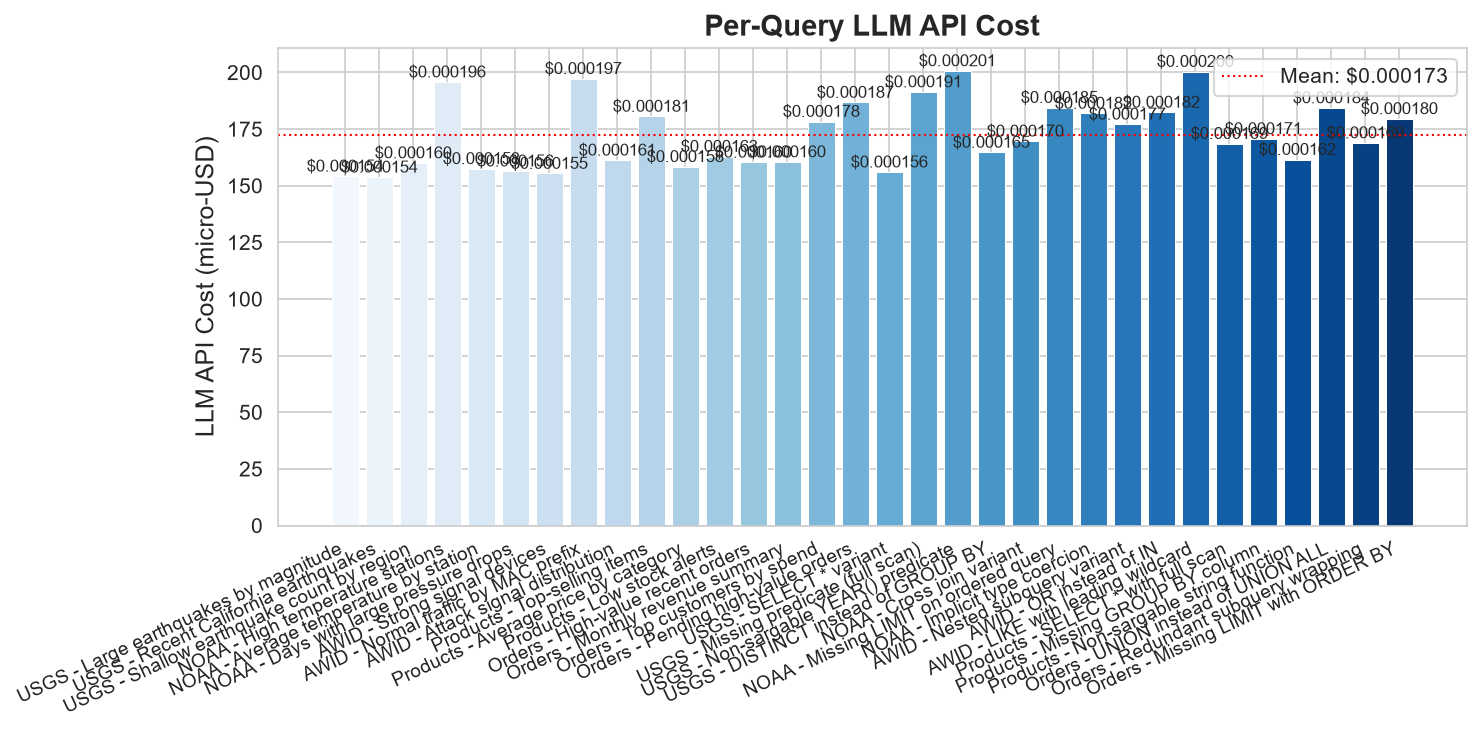
\includegraphics[width=0.90\linewidth]{../figures/llm_cost_breakdown.png}
\caption{Per-query LLM API cost in micro-USD (N=32).}
\label{fig:cost}
\end{figure}

\noindent\textbf{Projected costs at scale.} At GPT-4o-mini pricing, analyzing 10{,}000 queries costs approximately \$1.74. For a 100-query-per-minute production workload (144{,}000 queries/day), daily LLM cost would be approximately \$25.06. Even at GPT-4o pricing (\$5.00/M input tokens, \$15.00/M output tokens), daily cost for the same workload would be approximately \$288.00. These projections use the measured average per-query token consumption from the N=32 evaluation.

\subsection{Scalability Considerations}
\label{sec:scalability}
While the evaluation uses 500-row tables, the framework's architecture supports horizontal scaling along several dimensions. (1) \textbf{Query execution}: individual query invocations against DuckDB are independent and can be parallelized with thread-level concurrency. (2) \textbf{LLM analysis}: API calls are embarrassingly parallel, although any larger deployment remains subject to provider rate limits and budget constraints. (3) \textbf{Persistence}: the SQLite backend can be replaced with PostgreSQL or a cloud-hosted database for concurrent multi-user access without schema changes. (4) \textbf{Data volume}: the framework accepts tables of arbitrary size; the 500-row constraint affects only this demonstration, not the architecture.

\section{Discussion}
The pilot demonstrates that LLMs can serve as query-review assistants when embedded in an execution and validation harness. The framework does not assume the model is correct; it treats model output as a recommendation that must be stored, executed, and checked. This is important for big data environments where silent result drift can be more damaging than a slow query.

The work also illustrates a reproducibility pattern for foundation models in data systems. Rather than reporting only model responses, the artifact captures prompts, scores, token counts, cost, rewrites, execution outcomes, and validation status. The rule-based comparison in Table~\ref{tab:rulebased} also clarifies the contribution: deterministic checks are enough for obvious patterns, while the LLM adds explanation and rewrite guidance when query structure is more context dependent.

The single false negative is instructive rather than problematic. The UNION-based query scored below the threshold because the model treated it as a relatively mild optimization issue, and that judgment is defensible in a pilot setting. More importantly, the missing GROUP BY case shows why execution-based validation is necessary: the framework did not accept the rewrite blindly, and the validator surfaced the ambiguity.

\section{Limitations and Future Work}
\label{sec:limitations}
\textbf{Pilot scale.} The experiment used 32 queries and 500-row tables. The 95\% confidence interval for accuracy (83.8\%--99.9\%) is substantially narrower than the N=8 pilot (63.1\%--100\%), but still wider than a production-grade benchmark. A production-credible evaluation would require approximately 385 queries for $\pm5\%$ margin. Until then, all performance claims must be interpreted as feasibility evidence for the architecture.

\textbf{Engine scope.} Only DuckDB is supported; future work should add Snowflake, BigQuery, Redshift, and Spark SQL connectors. \textbf{Validation depth.} Row-count and checksum comparison does not prove full SQL equivalence. \textbf{LLM dependency.} Cost and quality depend on the configured model.

Future work should expand the query corpus beyond 100 queries, evaluate multiple LLMs (GPT-4o, Claude, Gemini, open-source models), test larger datasets (10K--1M rows), and study reviewer-facing explanations for big data governance under the 5V framework (volume, velocity, variety, veracity, value).

\section{Conclusion}
This paper presented a reproducible framework for LLM-powered SQL query monitoring and optimization in big data environments. The framework integrates public dataset ingestion, controlled DuckDB workload execution, persistent SQLite query-history storage, structured LLM-based analysis with a defined prompt template, automated rewrite generation, execution-based tested-instance result validation through row-count and checksum comparison, and comprehensive cost accounting. Each deterministic stage is independently executable, and all model outputs are auditable through the shared SQLite database.

We evaluated the framework on a workload of 32 queries (16 baseline and 16 inefficient variants) across five datasets spanning scientific, environmental, cybersecurity, and commercial domains, targeting 12 anti-pattern types. The LLM analyzer achieved 96.9\% detection accuracy (31/32), 0\% false positive rate (0/16), and 93.8\% recall (15/16). The single false negative---a UNION-based variant---is a minor anti-pattern appropriately scored below the detection threshold. Fourteen of fifteen rewrites preserved tested-instance result equivalence (93.3\% result-equivalence rate). Total LLM API cost was \$0.005522 for all 32 analyses, or approximately \$0.000173 per query.

The results should be interpreted as evidence of feasibility, not as production-scale performance claims. With N=32, the 95\% confidence interval for detection accuracy narrows to [83.8\%, 99.9\%]---a 56\% reduction in half-width compared to an earlier N=8 pilot---but remains wider than a production-grade benchmark. The contribution is the framework itself: a modular, auditable artifact that can be extended, benchmarked, and compared against future approaches by the research community.

Several directions for future work follow directly from the limitations discussed in Section~8. Expanding the query corpus beyond 100 queries, evaluating multiple LLMs (GPT-4o, Claude, Gemini, open-source models), testing larger datasets (10K--1M rows), extending the execution engine layer to support Snowflake, BigQuery, Redshift, and Spark SQL, and studying the human-facing presentation of LLM-based query reviews would each strengthen the framework's applicability to production big data governance under the 5V framework (volume, velocity, variety, veracity, value).

\subsection*{Reproducibility Statement}
The complete framework, including all source code, dataset download scripts, workload definitions, prompt templates, analysis outputs, and documentation, is publicly available at~\cite{sharma2026framework}. The artifact is distributed with a README describing installation, execution, and reproduction of all results reported in this paper.

\bibliographystyle{IEEEtran}
\bibliography{references}

\end{document}





